\documentclass[12pt,letterpaper]{article}

% APA 7 formatting packages
\usepackage[utf8]{inputenc}
\usepackage[margin=1in]{geometry}
\usepackage{amsmath,amsfonts,amssymb}
\usepackage{graphicx}
\usepackage{cite}
\usepackage{url}
\usepackage{booktabs}
\usepackage{array}
\usepackage{enumitem}
\usepackage{fancyhdr}
\usepackage{titlesec}
\usepackage{xcolor}
\usepackage{listings}
\usepackage{float}
\usepackage{microtype}
\usepackage{setspace}
\usepackage{tocloft}
\usepackage{tikz}
\usetikzlibrary{shapes,arrows,positioning,chains}

% APA 7 compliant formatting
\doublespacing
\setlength{\parindent}{0.5in}

% APA 7 style headers and footers
\pagestyle{fancy}
\fancyhf{}
\setlength{\headheight}{15pt}
\fancyhead[R]{\thepage}
\renewcommand{\headrulewidth}{0pt}

% APA 7 title formatting
\titleformat{\section}[hang]{\normalfont\bfseries\centering}{\thesection}{1em}{}
\titleformat{\subsection}[hang]{\normalfont\bfseries}{\thesubsection}{1em}{}
\titleformat{\subsubsection}[hang]{\normalfont\bfseries}{\thesubsubsection}{1em}{}

% Table of Contents formatting
\renewcommand{\cftsecleader}{\cftdotfill{\cftdotsep}}
\setcounter{tocdepth}{3}

\begin{document}

% APA 7 Title Page
\begin{titlepage}
    \centering
    \vspace*{2in}
    
    {\large\bfseries Nebula GPU Interconnect System: Implementation Status and Architecture Analysis}
    
    \vspace{2in}
    
    Pranav Chandra, Pramit Pal, Meghadri Ghosh\\
    Team Bob\\
    
    \vspace{1in}
    
    Technical Implementation Report\\
    
    \vspace{1in}
    
    September 10th, 2025
    
\end{titlepage}

% Table of Contents
\newpage
\pagenumbering{roman}
\tableofcontents
\newpage

% Abstract on separate page
\section*{Abstract}
\addcontentsline{toc}{section}{Abstract}

This technical report documents the current implementation status of the Nebula GPU interconnect system. The system implements a Network-on-Chip (NoC) architecture for multi-GPU communication with support for AXI4 and CHI coherency protocols. The implementation includes a five-stage router pipeline, protocol translation components, mesh topology generation, and testing infrastructure. The report describes the architectural components, implementation details, and verification framework based on the SystemVerilog RTL code and supporting tools.

\newpage
\pagenumbering{arabic}

{\color{red}\section*{\large\bfseries DISCLAIMER: AI USAGE}}
\addcontentsline{toc}{section}{Disclaimer: AI Usage}

The organizers of the Astera Labs challenge should be informed that this submission utilized AI tools to improve and work upon the overall code base. Although the architecture and the planning of the overall submission was ideated by the team members, a non-negligible proportion of the code base was made with the help of AI tools. The basic implementation and debugging as well as understanding of the code is present with the team.

\section{Introduction}

The Nebula system is a hardware-based interconnect implementation for GPU communication. The design targets deterministic, low-latency communication between GPU nodes arranged in a 2D mesh topology. The system includes support for non-coherent AXI4 transactions and coherent CHI protocol operations.

The current implementation covers the core functionality with some advanced features in development. The remaining work includes enhancements to adaptive routing algorithms and quality-of-service features.

\section{System Architecture}

\subsection{Overall Topology}

The system implements a parameterizable 2D mesh topology supporting grid sizes from 2×2 to 8×8 nodes. Each node in the mesh contains a router with five bidirectional ports (North, South, East, West, Local) and supports connection to external GPU interfaces.

The mesh topology is generated through the \texttt{nebula\_mesh\_top.sv} module, which automatically handles router instantiation and interconnection. Edge nodes are properly terminated with tie-off logic for unused ports. Figure \ref{fig:component-architecture} illustrates the overall system architecture and component relationships within the Nebula interconnect system.

\begin{figure}[H]
    \centering
    \includegraphics[width=0.6\textwidth]{images/component-architecture.png}
    \caption{Nebula System Component Architecture}
    \label{fig:component-architecture}
\end{figure}

The system supports 3×3 mesh topology configurations with router interconnections and port assignments.

\subsection{Router Microarchitecture}

The router implementation (\texttt{nebula\_router.sv}) follows a five-stage pipeline architecture:

\begin{enumerate}
    \item \textbf{Buffer Write (BW)}: Input port management and virtual channel allocation
    \item \textbf{Route Computation (RC)}: XY routing algorithm with destination coordinate extraction
    \item \textbf{Virtual Channel Allocation (VA)}: VC state machines and downstream VC allocation
    \item \textbf{Switch Allocation (SA)}: Crossbar arbitration with round-robin scheduling
    \item \textbf{Switch Traversal (ST)}: Crossbar switching and credit management
\end{enumerate}

Each router supports four virtual channels per input port with 16-flit depth FIFO buffers. The implementation includes credit-based flow control and round-robin arbitration for fairness. Figure \ref{fig:inter-router-comms} shows the inter-router communication protocols and data flow mechanisms.

\begin{figure}[H]
    \centering
    \includegraphics[width=0.8\textwidth]{images/inter-router-comms.png}
    \caption{Inter-Router Communication and Data Flow}
    \label{fig:inter-router-comms}
\end{figure}

The router follows a five-stage pipeline architecture with data flow between stages.

\subsubsection{Buffer Write Stage Implementation}

The Buffer Write (BW) stage is implemented in lines 135-180 of \texttt{nebula\_router.sv} and handles incoming network traffic at input ports. The stage manages virtual channel allocation and flow control through combinational logic that checks buffer availability across virtual channels before accepting incoming flits.

The implementation includes a buffer availability check that iterates through four virtual channels per input port, examining \texttt{vc\_full[g\_port][g\_vc]} signals to determine available space. When a flit arrives via \texttt{flit\_in\_valid}, the stage extracts the virtual channel identifier from the flit header (\texttt{flit\_in.vc\_id}) and validates buffer space availability before enabling the write operation. The ready signal (\texttt{flit\_in\_ready}) is asserted when the system has completed reset and at least one virtual channel has available buffer space.

The flit write operation uses dedicated FIFO instances for each virtual channel, with \texttt{vc\_write\_en[g\_port][g\_vc]} controlling data insertion and \texttt{vc\_write\_data} carrying the flit payload. The stage includes debug logging that records flit acceptance events with routing information including coordinates, flit type, and virtual channel assignment. The implementation follows credit-based flow control protocols for network operation.

\subsubsection{Route Computation Stage Implementation}

The Route Computation (RC) stage is implemented in lines 260-380 of \texttt{nebula\_router.sv} and handles routing algorithm execution. The stage processes head and single flits from virtual channel buffers using show-ahead FIFO functionality for data access without explicit read operations.

The routing logic implements XY dimension-ordered routing, which provides deadlock freedom through ordered path selection. The algorithm compares the destination X-coordinate (\texttt{current\_flit.dest\_x}) with the current router's X-coordinate (\texttt{ROUTER\_X}), directing flits east or west as needed. After reaching the correct X-coordinate, the algorithm routes flits north or south until destination coordinates match. When coordinates align (\texttt{current\_flit.dest\_x == ROUTER\_X \&\& current\_flit.dest\_y == ROUTER\_Y}), the routing logic directs flits to the local port.

The implementation includes adaptive routing extensions that incorporate congestion monitoring for path selection in non-boundary cases. The system calculates congestion metrics using buffer utilization, credit counts, and virtual channel statistics across output ports. When congestion exceeds a threshold (implemented as a configurable parameter), the adaptive logic considers alternative paths while maintaining deadlock freedom. The decision mechanism includes hysteresis to prevent route oscillation during varying congestion conditions.

\subsubsection{Virtual Channel Allocation Stage Implementation}

The Virtual Channel Allocation (VA) stage is implemented in lines 390-450 of \texttt{nebula\_router.sv} and manages downstream virtual channel assignment for packets. The stage operates between route computation and switch allocation, handling virtual channel resource allocation while maintaining fairness across the network.

The allocation algorithm uses a sequential approach that evaluates available output virtual channels for the target output port determined by the RC stage. The process begins when \texttt{rc\_valid[g\_port][g\_vc]} indicates successful route computation, triggering examination of credit availability across output virtual channels. The implementation checks \texttt{credit\_count[rc\_out\_port][selected\_vc]} counters to verify downstream buffer space before committing to virtual channel allocation.

The allocation decision iterates through virtual channels in order, selecting the first available VC that meets credit requirements. Upon successful allocation, the stage updates state registers including \texttt{va\_out\_port} and \texttt{va\_out\_vc} to record the allocation decision, while updating virtual channel state machine variables \texttt{vc\_out\_port} and \texttt{vc\_out\_vc} for subsequent pipeline stages. The implementation includes debug logging that tracks allocation events, providing visibility into virtual channel utilization and credit availability. The approach maintains credit-based flow control semantics for preventing buffer overflow.

\subsubsection{Switch Allocation Stage Implementation}

The Switch Allocation (SA) stage is implemented in lines 460-570 of \texttt{nebula\_router.sv} and handles crossbar arbitration for access to output ports while managing backpressure conditions and maintaining fairness across competing virtual channels. The stage coordinates between multiple arbitration units and includes grant tracking for operation under congested network conditions.

The arbitration mechanism uses dedicated round-robin arbiters (\texttt{nebula\_rr\_arbiter}) instantiated for each output port, with each arbiter managing up to twenty requestors (four virtual channels across five input ports). The arbitration process evaluates requests from virtual channels that have completed virtual channel allocation and have sufficient downstream credits for packet transmission. The round-robin scheduling algorithm provides fair access to output resources, preventing any single virtual channel from monopolizing bandwidth.

The implementation includes grant persistence tracking for backpressure handling. The \texttt{granted\_but\_blocked} registers maintain state information for virtual channels that won arbitration but encountered downstream backpressure conditions. The system prioritizes these persistent blocked grants over new arbitration requests, so packets experiencing temporary backpressure receive treatment once downstream resources become available. This mechanism addresses resource starvation scenarios that could occur under sustained network congestion. The arbitration request generation logic combines current virtual channel allocation validity (\texttt{va\_valid}) with credit availability checks, so only viable transmission requests participate in the arbitration process.

\subsubsection{Switch Traversal Stage Implementation}

The Switch Traversal (ST) stage is implemented in lines 580-620 of \texttt{nebula\_router.sv} and serves as the final pipeline stage responsible for coordinating data transmission across the router's crossbar switch while maintaining protocol compliance and credit management. The stage transforms arbitration decisions from the SA stage into flit transmission operations, so only authorized and resource-verified packets proceed to their designated output ports.

The output valid signal generation logic (\texttt{flit\_out\_valid}) requires simultaneous satisfaction of multiple conditions before asserting packet transmission validity. The stage verifies that the current virtual channel has won switch arbitration through the SA stage grants, confirms that sufficient downstream buffer space remains available through credit tracking mechanisms, and validates that the downstream router or interface can accept the incoming flit via ready signal assertion. This verification approach prevents protocol violations and maintains network stability under varying operational conditions.

The flit modification process updates the virtual channel identifier field within outgoing flits to reflect the downstream virtual channel assignment determined during the VA stage. The \texttt{vc\_out\_vc} assignment allows receiving routers to properly categorize incoming flits according to their local virtual channel management schemes. The stage implements backpressure propagation through ready signal management, where upstream flow control signals reflect downstream resource availability. The credit management integration coordinates with dedicated credit flow control modules to maintain accounting of buffer utilization across virtual channel boundaries.

\subsubsection{Virtual Channel State Machine}

The Virtual Channel State Machine is implemented in lines 630-690 of \texttt{nebula\_router.sv} and manages the lifecycle of individual virtual channels from packet arrival through transmission, handling resource allocation and deallocation while maintaining network flow control semantics. Each virtual channel maintains independent state tracking to support concurrent packet processing across multiple traffic flows.

The state machine implements a four-state progression: IDLE → ROUTING → WAITING\_VC → ACTIVE → IDLE, with each transition triggered by specific pipeline stage completion events. The IDLE state represents an unallocated virtual channel awaiting packet arrival, transitioning to ROUTING upon receiving a head or single flit that requires destination analysis. The ROUTING state persists until the Route Computation stage determines the appropriate output port, at which point the state advances to WAITING\_VC to await virtual channel allocation completion. The WAITING\_VC state concludes when the Virtual Channel Allocation stage secures downstream resources, enabling transition to the ACTIVE state where packet transmission occurs.

The state transition logic incorporates pipeline stage coordination through validation signals including \texttt{rc\_valid}, \texttt{va\_valid}, and successful switch arbitration indicators. The ACTIVE state management includes packet completion detection that monitors flit types to identify TAIL or SINGLE flits, indicating the end of packet transmission and triggering return to the IDLE state for resource reclamation. The implementation includes \texttt{vc\_read\_en} signal generation that coordinates with FIFO buffer interfaces for proper data flow timing. The state machine incorporates debug logging mechanisms that provide visibility into virtual channel utilization patterns for performance analysis and network optimization efforts.

The virtual channel state machine manages transitions and conditions for state changes.

\subsubsection{Credit Management Implementation}

The Credit Management system is implemented in lines 700-750 of \texttt{nebula\_router.sv} and provides the flow control mechanism that prevents buffer overflow conditions while enabling throughput utilization across the network topology. The subsystem uses dedicated \texttt{nebula\_credit\_flow\_ctrl} module instances for each output virtual channel, creating a distributed credit tracking architecture that maintains accounting of downstream buffer availability.

Each credit controller maintains a counter that tracks available buffer space in the corresponding downstream virtual channel, with the maximum credit count configured to match the virtual channel buffer depth of 16 flits as specified in \texttt{nebula\_pkg.sv}. The credit increment mechanism activates upon successful flit transmission, indicated by the simultaneous assertion of \texttt{flit\_out\_valid} and \texttt{flit\_out\_ready} signals along with appropriate virtual channel identifier matching. This increment operation reflects the freeing of one buffer slot in the downstream router, making that capacity available for future packet transmission.

The credit decrement process occurs during the Virtual Channel Allocation stage when a virtual channel secures downstream resources. The \texttt{va\_valid} signal assertion, combined with matching output port and virtual channel identifiers, triggers credit consumption that reserves downstream buffer space for the allocated packet. This credit reservation mechanism provides packets accepted for transmission with guaranteed downstream resources, preventing deadlock scenarios that could arise from resource allocation conflicts. The credit availability signals (\texttt{credits\_available}) provide feedback to the allocation and arbitration stages for resource management decisions.

\section{Packet Format and Protocol}

\subsection{Flit Structure}

The Nebula system implements a 256-bit flit-based packet format defined in \texttt{nebula\_pkg.sv} that includes payload data and header information required for network operation. The flit structure represents the basic data unit transmitted across the network, incorporating routing information, flow control parameters, and error detection within a fixed-width format.

The flit type classification uses a 2-bit encoding scheme that supports four flit categories: HEAD (00), BODY (01), TAIL (10), and SINGLE (11). This classification enables multi-flit packet support while providing packet boundary demarcation for virtual channel state machine operation. HEAD flits carry routing header information and initiate packet transmission, while BODY flits transport additional payload data for larger packets. TAIL flits provide packet termination signaling with final payload content, and SINGLE flits combine header and complete payload for single-flit packets.

The virtual channel identification field uses 2 bits to specify one of four virtual channels per port, supporting CHI protocol requirements with dedicated channels for requests (VC\_REQ), responses (VC\_RSP), snoops (VC\_SNP), and data transfers (VC\_DAT). The coordinate fields allocate 4 bits each for source and destination X/Y coordinates, enabling mesh topologies up to 16×16 routers. The 16-bit sequence number field provides packet ordering capabilities for maintaining coherency protocol semantics, while the 8-bit packet identifier enables transaction tracking across protocol boundaries.

The flit structure shows the detailed bit allocation within a 256-bit flit, with header fields and payload organization.

Quality-of-Service (QoS) support uses 4 bits to classify traffic into sixteen priority levels for differentiated service delivery. The 208-bit payload field provides data transmission capacity while accommodating the 48-bit header overhead. Error detection uses a 32-bit Cyclic Redundancy Check (CRC) field that provides protection against transmission errors throughout the network fabric. The flit structure supports packet transmission across the Nebula interconnect architecture.

\subsection{Packet Assembly and Disassembly}

The packet handling infrastructure is implemented through \texttt{nebula\_packet\_assembler.sv} and \texttt{nebula\_packet\_disassembler.sv} and provides mechanisms for converting between high-level protocol transactions and the flit-based network format required for NoC transmission. These modules serve as protocol translation layers that handle multi-flit packet management while maintaining data integrity throughout the transmission process.

The packet assembler module implements multi-flit packet support with configurable flit-per-packet ratios that adapt to varying payload sizes and protocol requirements. The header generation subsystem extracts routing coordinates from high-level address information, mapping global memory addresses to appropriate mesh coordinates through address translation functions. This process includes destination coordinate calculation, source coordinate injection based on the originating router location, and virtual channel assignment according to protocol message classification schemes. The payload segmentation algorithm distributes large data transfers across multiple flits while maintaining proper packet boundaries and utilizing the available payload capacity within each flit.

The packet disassembly process operates in reverse, reconstructing complete high-level transactions from sequences of received flits while validating packet integrity and maintaining proper ordering semantics. The module implements CRC verification mechanisms that detect transmission errors and trigger appropriate error recovery procedures. The sequence number management system provides correct packet ordering even when multiple packets traverse different network paths or experience varying latencies due to congestion or adaptive routing decisions. The disassembler maintains transaction state information to handle multi-flit packet reconstruction, coordinating with virtual channel state machines for proper resource management throughout the reassembly process.

\section{Protocol Interface Implementation}

\subsection{AXI4 Interface}

The AXI4 interface implementation (\texttt{nebula\_niu\_axi.sv}, \texttt{nebula\_axi\_if.sv}) provides complete support for all five AXI4 channels:

\subsubsection{AXI4 State Machines}

The AXI4 interface implementation spans \texttt{nebula\_niu\_axi.sv} and \texttt{nebula\_axi\_if.sv} and provides support for all five AXI4 communication channels through dedicated state machine implementations that manage concurrent transaction processing while maintaining protocol compliance. The interface architecture implements separate state machines for each channel to enable throughput and minimize latency through parallel operation.

The Address Write (AW) channel state machine is implemented in lines 130-180 of \texttt{nebula\_axi\_if.sv} and manages the write address phase through a four-state progression: AW\_IDLE → AW\_WAIT\_DATA → AW\_SEND\_REQ → AW\_WAIT\_RESP. The AW\_IDLE state monitors for incoming write address requests, transitioning to AW\_WAIT\_DATA upon receiving valid address information. The AW\_WAIT\_DATA state coordinates with the Write Data (W) channel to provide synchronized address and data transmission, preventing protocol violations that could arise from mismatched address and data phases. Upon confirming data availability, the state machine advances to AW\_SEND\_REQ for address transmission, concluding with AW\_WAIT\_RESP to await write completion confirmation.

The Write Data (W) channel implements a three-state machine: W\_IDLE → W\_DATA → W\_WAIT\_LAST, designed to handle burst write operations with beat counting and boundary management. The state machine tracks individual data beats within a burst transaction, monitoring the WLAST signal to detect burst completion. The Write Response (B) channel uses a two-state approach: B\_IDLE → B\_RESP, managing write completion acknowledgments and error status reporting.

The Address Read (AR) and Read Data (R) channels implement state machines optimized for read transaction characteristics. The AR channel follows AR\_IDLE → AR\_SEND\_REQ → AR\_WAIT\_RESP progression, while the R channel operates through R\_IDLE → R\_DATA states with burst completion detection. Each state machine incorporates error handling mechanisms, timeout detection, and performance monitoring capabilities for operation under diverse network conditions.

\subsubsection{Outstanding Transaction Management}

The Outstanding Transaction Management subsystem is implemented in lines 100-130 of \texttt{nebula\_axi\_if.sv} and provides tracking capabilities for concurrent AXI4 transactions that enable operation while maintaining protocol ordering requirements and resource allocation. The system uses a dedicated transaction table with 64 entries, configured to support the throughput requirements of GPU workloads that generate concurrent memory access requests.

The transaction table architecture employs a structured approach where each entry contains transaction metadata including AXI identifier fields, address information, burst parameter specifications, and transaction timing data. The \texttt{transaction\_entry\_t} structure incorporates fields for tracking burst length, burst type classification (FIXED, INCR, WRAP), transfer size encoding, and quality-of-service parameters. Each entry maintains state information regarding transaction progression, enabling the interface to coordinate between request initiation and response completion across network latencies.

The table management algorithms implement FIFO-style operation through dedicated write and read pointer mechanisms (\texttt{outstanding\_wr\_ptr}, \texttt{outstanding\_rd\_ptr}) that provide proper transaction ordering while preventing resource conflicts. The allocation process occurs during transaction initiation, when the interface assigns a table entry to track the newly initiated request. The \texttt{alloc\_valid} signal indicates successful entry allocation, while the \texttt{outstanding\_full} flag provides backpressure signaling when the table reaches capacity limits.

Transaction completion handling uses lookup algorithms that match incoming responses with their corresponding outstanding requests through transaction identifier correlation. The lookup process examines the \texttt{noc\_resp\_flit.packet\_id} field against stored transaction identifiers, enabling response routing even when transactions complete out-of-order due to network timing variations. The \texttt{lookup\_valid} signal confirms successful transaction matching, triggering entry deallocation and resource reclamation.

\subsubsection{Burst Decomposition}

Burst handling (\texttt{nebula\_axi\_noc\_bridge.sv}, lines 120-180):

\begin{itemize}
    \item Supports FIXED, INCR, and WRAP burst types
    \item Burst length up to 256 beats
    \item Address calculation for each beat
    \item Beat counting and last beat detection
\end{itemize}

\subsection{CHI Coherency Protocol}

The CHI implementation (\texttt{nebula\_chi\_interface.sv}, \texttt{nebula\_chi\_directory.sv}) supports:

\subsubsection{CHI Directory Controller}

The CHI Directory Controller, implemented in lines 90-130 of \texttt{nebula\_chi\_directory.sv}, serves as the central coherency management engine that coordinates cache line ownership and sharing information across the distributed GPU cluster architecture. The controller implements a finite state machine with nine distinct states that manage the complete lifecycle of coherency transactions from initial request reception through final completion acknowledgment, ensuring adherence to the CHI protocol specifications while optimizing for GPU workload characteristics.

The directory controller's state machine progression follows the sequence: 
IDLE → LOOKUP → SNOOP\_BROADCAST → AWAIT\_SNOOP\_RESP → MEMORY\_ACCESS → DATA\_TRANSFER → UPDATE\_DIRECTORY → SEND\_COMPLETION → ERROR\_RECOVERY. 

The IDLE state monitors for incoming coherency requests, transitioning to LOOKUP upon receiving valid CHI transaction initiation. The LOOKUP state examines the 2048-entry directory cache to determine current cache line ownership and sharing status, utilizing the address-based indexing scheme that maps memory addresses to directory entries through configurable hash functions.

The SNOOP\_BROADCAST state coordinates with remote cache controllers by generating appropriate snoop messages to all potential sharers identified in the directory entry's sharer bit vector. The controller maintains sharer tracking through a 64-bit vector that supports mesh topologies up to 64 nodes, with each bit position corresponding to a specific router coordinate within the network. The AWAIT\_SNOOP\_RESP state implements timeout-based snoop response collection with a configurable 1024-cycle timeout period, preventing indefinite blocking due to failed or non-responsive cache controllers.

Memory access coordination occurs during the MEMORY\_ACCESS state, where the controller generates appropriate memory subsystem requests for cache line data retrieval or writeback operations. The DATA\_TRANSFER state manages the movement of cache line data between requesting nodes, memory subsystems, and sharing caches according to the determined coherency action. The UPDATE\_DIRECTORY state modifies directory entries to reflect the new ownership and sharing configuration resulting from the transaction, while SEND\_COMPLETION generates appropriate CHI completion responses to satisfy protocol requirements. The ERROR\_RECOVERY state handles exceptional conditions including snoop timeouts, memory access failures, and protocol violations, implementing appropriate recovery mechanisms to maintain system stability and data integrity.

\subsubsection{CHI Message Types}

The CHI protocol implementation supports a set of transaction types defined in lines 106-120 of \texttt{nebula\_chi\_directory.sv}, encompassing the essential coherency operations required for cache-coherent GPU cluster operation. The message type classification system provides the foundation for maintaining data consistency across distributed cache hierarchies while enabling high-performance concurrent access to shared memory regions.

The READ\_SHARED transaction type implements non-exclusive read access that allows multiple cache controllers to maintain shared copies of the same cache line, optimizing read-intensive workloads common in GPU computational kernels. The transaction preserves existing sharing relationships while ensuring that all sharers receive consistent data. READ\_UNIQUE transactions provide exclusive read access that invalidates all other cached copies, preparing cache lines for subsequent modification while maintaining coherency invariants. These transactions coordinate through the directory controller to identify and invalidate remote cached copies before granting exclusive access to the requesting node.

WRITE\_UNIQUE operations represent the most complex transaction type, requiring coordination between the directory controller, existing cache line owners, and memory subsystems to ensure atomic update semantics. The implementation validates current ownership status, coordinates with sharing caches to invalidate stale copies, and manages the transition of exclusive ownership to the requesting node. WRITEBACK transactions handle the controlled eviction of modified cache lines, ensuring that dirty data reaches the memory subsystem before cache line replacement occurs. EVICTION operations manage cache line replacement for unmodified data, coordinating with the directory controller to update sharing vectors appropriately.

SNOOP\_RESP transactions provide the response mechanism for distributed coherency coordination, enabling remote caches to communicate ownership status, data availability, and cache line state information to the requesting directory controller. ATOMIC transactions support hardware-accelerated atomic memory operations essential for GPU synchronization primitives, implementing compare-and-swap, fetch-and-add, and other atomic semantics through coordinated directory and cache controller interaction. This transaction type support ensures that the CHI implementation can manage the diverse coherency requirements of modern GPU computing workloads while maintaining the performance characteristics essential for high-throughput parallel processing applications.

\subsubsection{Directory Entry Structure}

The Directory Entry Structure, defined in lines 230-240 of \texttt{nebula\_pkg.sv}, implements a cache line metadata storage format that captures all information necessary for maintaining coherency across the distributed GPU cluster architecture. Each directory entry represents a complete cache line state record that enables the directory controller to make informed coherency decisions while minimizing metadata overhead and access latency.

The cache state field utilizes the industry-standard MOESI (Modified, Owned, Exclusive, Shared, Invalid) cache coherency protocol encoding that provides optimal balance between coherency overhead and performance characteristics for GPU workloads. The Modified state indicates that a single cache holds the only valid, modified copy of the cache line, requiring writeback coordination during subsequent access requests. The Owned state represents a cache that holds a modified copy while allowing shared read access by other caches, optimizing read-sharing scenarios for frequently accessed data structures. The Exclusive state provides single-cache ownership without modification, enabling efficient transition to Modified state for subsequent writes. The Shared state allows multiple caches to maintain read-only copies, while the Invalid state indicates absent or outdated cache line copies.

The owner node identifier employs 6 bits to specify the current exclusive or owned cache controller within mesh topologies supporting up to 64 nodes, providing direct lookup capability for ownership transfer operations. The sharer bit vector utilizes 64 bits to maintain a map of all caches that possess shared copies of the cache line, enabling efficient snoop broadcast optimization through selective targeting of relevant cache controllers rather than network-wide broadcasts.

The dirty bit indicates whether the cache line contains modifications relative to the memory subsystem, coordinating writeback requirements during ownership transfers and eviction operations. The valid bit provides entry allocation status, distinguishing between active directory entries and available storage slots within the directory cache structure. The pending transaction identifier field, utilizing the full CHI transaction ID width, enables the directory controller to coordinate multiple concurrent operations on the same cache line while preventing race conditions and ensuring atomic transaction semantics. This directory entry structure provides the metadata foundation necessary for reliable, high-performance coherency management across large-scale GPU cluster deployments.

\subsection{Protocol Translation}

Two bridge modules handle protocol translation:

\subsubsection{AXI-NoC Bridge}

The AXI-NoC bridge (\texttt{nebula\_axi\_noc\_bridge.sv}) implements:

\begin{itemize}
    \item 64-entry reorder buffer for response reconstruction
    \item Burst decomposition with address calculation
    \item Packet ID generation and tracking
    \item Latency measurement and buffer utilization monitoring
\end{itemize}

\subsubsection{CHI-NoC Bridge}

The CHI-NoC bridge (\texttt{nebula\_chi\_noc\_bridge.sv}) provides:

\begin{itemize}
    \item CHI message classification and VC mapping
    \item Coherency state preservation across NoC transport
    \item Snoop response aggregation
    \item Directory update coordination
\end{itemize}

\section{Common Infrastructure}

\subsection{FIFO Buffer Implementation}

The FIFO implementation (\texttt{nebula\_fifo.sv}) provides:

\begin{itemize}
    \item Parameterizable data width (default: 256 bits) and depth (default: 16)
    \item Show-ahead read mode (data available without read enable)
    \item Full/empty flag generation with almost\_full/almost\_empty
    \item Count output for buffer utilization tracking
    \item Synchronous read/write pointers with wraparound
\end{itemize}

\subsection{Round-Robin Arbiter}

The arbiter (\texttt{nebula\_rr\_arbiter.sv}) implements:

\begin{itemize}
    \item Priority mask-based round-robin scheduling
    \item Parameterizable number of requestors (default: 20 for 5 ports × 4 VCs)
    \item One-hot grant output with grant ID
    \item Priority encoder for masked and unmasked requests
\end{itemize}

\subsection{Credit Flow Control}

Credit management (\texttt{nebula\_credit\_flow\_ctrl.sv}) provides:

\begin{itemize}
    \item Configurable maximum credits (default: 16)
    \item Credit increment on downstream acceptance
    \item Credit decrement on flit transmission
    \item Credits\_available signal generation
\end{itemize}

\section{System Integration}

\subsection{Top-Level Modules}

The system integration is handled through hierarchical modules:

\subsubsection{Nebula System Top}

\texttt{nebula\_system\_top.sv} provides:

\begin{itemize}
    \item AXI4 interfaces for all nodes in the mesh
    \item Global address mapping with configurable base addresses
    \item Node coordinate calculation functions
    \item System-wide performance monitoring
\end{itemize}

\subsubsection{Nebula Mesh Top}

\texttt{nebula\_mesh\_top.sv} implements:

\begin{itemize}
    \item Parameterized router instantiation (2×2 to 8×8)
    \item Automatic interconnection logic for mesh topology
    \item Edge node handling with unused port termination
    \item VC status and performance counter aggregation
\end{itemize}

\subsubsection{Nebula Top}

\texttt{nebula\_top.sv} includes:

\begin{itemize}
    \item Configuration register interface (256 registers)
    \item System status and error reporting
    \item Performance counter aggregation
    \item Debug and trace interfaces
\end{itemize}

\subsection{Address Mapping}

Address-to-coordinate mapping (\texttt{nebula\_niu\_axi.sv}, lines 130-180):

\begin{itemize}
    \item 64-bit global address space support
    \item Configurable node address ranges (default: 1MB per node)
    \item Local vs. remote access determination
    \item Boundary validation with error reporting
\end{itemize}


\subsection{Python Analysis Tools}

The Nebula system includes a comprehensive suite of Python-based analysis tools located in the \texttt{python/} directory that support simulation, verification, and performance analysis activities throughout the development and testing process. These tools form an integrated ecosystem that enables researchers and engineers to characterize network behavior, generate test scenarios, and analyze system performance under diverse operational conditions.

\subsubsection{Traffic Generator}

The traffic generation infrastructure is implemented in \texttt{nebula\_traffic\_generator.py} and serves as the primary mechanism for creating realistic workload scenarios that exercise the interconnect system under controlled conditions. The generator supports mesh configurations ranging from 2×2 to 8×8 topologies, allowing researchers to evaluate scalability characteristics across different network sizes. The implementation includes multiple traffic pattern generation algorithms, including uniform random distribution for baseline performance characterization, hotspot patterns that concentrate traffic on specific nodes to evaluate congestion handling, and CNN training workloads that emulate realistic deep learning computation and communication patterns.

The system generates SystemVerilog testbench files that integrate directly with the RTL simulation environment, enabling automated verification workflows that combine traffic generation with cycle-accurate hardware simulation. VCD trace generation capabilities provide detailed visibility into signal transitions and timing relationships, supporting both functional verification and performance analysis. The performance metric calculation subsystem processes simulation results to extract key indicators including latency distributions, throughput measurements, and resource utilization statistics.

\subsubsection{VCD Parser}

The VCD parsing infrastructure, implemented in \texttt{nebula\_vcd\_parser.py}, provides post-simulation analysis capabilities that extract meaningful performance data from VCD trace files generated during RTL simulation. The parser implements specialized algorithms for identifying router events, packet transmission sequences, and timing relationships within the complex signal traces produced by large-scale mesh simulations.

The packet event extraction mechanism analyzes VCD signals to reconstruct complete packet journeys from injection through delivery, maintaining timestamp accuracy and routing path information throughout the extraction process. This capability enables detailed analysis of individual packet behavior, including hop-by-hop latency measurements and congestion-induced delays. The performance analysis subsystem processes these extracted events to generate statistical summaries, latency histograms, and throughput characterizations across different traffic scenarios. The visualization components transform numerical data into graphical representations that facilitate understanding of network behavior patterns and performance trends.

\subsubsection{Web Dashboard}

The web-based dashboard system, implemented in \texttt{web\_dashboard/backend/app.py}, provides an interactive interface for real-time visualization and control of simulation experiments. The dashboard architecture combines a Flask-based backend with a modern web frontend to deliver responsive visualization capabilities that support both live simulation monitoring and post-simulation analysis workflows.

The mesh visualization component renders network topology with animated packet flow representations that enable intuitive understanding of traffic patterns and congestion formation. The VCD replay functionality includes speed control mechanisms that allow researchers to examine network behavior at different temporal granularities, from cycle-level detail to high-level trend analysis. Performance metric trending capabilities maintain historical data and generate time-series visualizations that capture system behavior evolution during extended simulation runs. The configuration control interface enables real-time parameter adjustment and simulation scenario modification, supporting interactive exploration of design space and performance optimization strategies.

\section{Performance Monitoring}

\subsection{Counters and Metrics}

The system implements performance monitoring:

\subsubsection{Router-Level Counters}

The router-level performance monitoring infrastructure, implemented in lines 780-822 of \texttt{nebula\_router.sv}, provides visibility into individual router operation through detailed counter mechanisms that track critical performance metrics and resource utilization patterns. This monitoring capability enables fine-grained analysis of network behavior, facilitating both runtime optimization and post-deployment performance characterization across diverse workload scenarios.

The packet routing counters maintain detailed statistics for each output port, tracking the total number of packets successfully forwarded through each direction (North, South, East, West, Local). This directional packet counting enables identification of traffic flow patterns and potential hotspot formation within the mesh topology, providing essential data for adaptive routing algorithm optimization and network load balancing decisions. The counters utilize sufficient bit width to prevent overflow during extended operation periods, ensuring accurate long-term performance measurement capabilities.

Virtual channel utilization monitoring provides critical insights into resource allocation efficiency and potential bottleneck identification. The implementation tracks per-virtual-channel occupancy levels, average utilization percentages, and peak usage statistics that enable administrators to optimize virtual channel allocation strategies for specific workload characteristics. The congestion level tracking incorporates both instantaneous measurements and historical averaging to provide understanding of traffic distribution patterns across the router's internal resources.

Buffer occupancy monitoring extends beyond simple utilization tracking to provide detailed analysis of buffer fill patterns, average occupancy levels, and peak usage scenarios. The credit count tracking provides real-time visibility into downstream resource availability, enabling identification of backpressure propagation patterns and potential flow control inefficiencies. The adaptive routing usage statistics quantify the frequency and effectiveness of congestion-aware path selection decisions, providing valuable feedback for algorithm tuning and optimization efforts. This router-level monitoring infrastructure creates the foundation for network management and performance optimization across the entire Nebula interconnect system.

\subsubsection{System-Level Monitoring}

The system-level monitoring infrastructure, implemented within \texttt{nebula\_top.sv}, provides network-wide visibility through aggregated performance metrics that enable holistic understanding of interconnect behavior and resource utilization across the entire mesh topology. This monitoring capability extends beyond individual router performance to capture system-wide trends, bottleneck identification, and overall network health assessment essential for large-scale GPU cluster management.

The total packet transmission and reception counters provide fundamental throughput measurements that quantify the overall data movement capacity of the interconnect system. These counters aggregate statistics from all routers within the mesh, providing system administrators with clear visibility into network utilization trends and capacity planning requirements. The implementation includes separate tracking for different packet types and priority classes, enabling detailed analysis of traffic composition and quality-of-service effectiveness.

Average latency measurement capabilities utilize timing mechanisms that track packet traversal times from injection through final delivery across various path lengths and congestion scenarios. The latency monitoring system maintains histograms of packet delivery times, enabling identification of tail latency scenarios and performance outliers that could impact application-level performance. The buffer utilization aggregation provides network-wide visibility into resource consumption patterns, identifying potential capacity constraints and enablingbling proactive resource allocation optimization.

Error counting and protocol violation detection mechanisms provide essential system health monitoring through tracking of transmission errors, protocol compliance failures, and resource allocation conflicts. The error classification system distinguishes between recoverable soft errors and serious protocol violations, enabling appropriate error handling and system recovery procedures. The performance counter integration includes mechanisms for counter overflow protection, periodic reset capabilities, and configurable sampling intervals that adapt to diverse monitoring requirements. This system-level monitoring infrastructure provides the visibility and analysis capabilities necessary for effective management of large-scale, high-performance GPU interconnect deployments.

\subsubsection{Dashboard Integration}

The web dashboard provides:

\begin{itemize}
    \item Real-time visualization of packet flows
    \item Performance metric graphing
    \item VCD trace replay with interactive controls
    \item Configuration parameter adjustment
\end{itemize}

\section{Implementation Status}

\subsection{Completed Components}

The Nebula GPU interconnect system has implemented the core architectural components with functionality verified through simulation and testing. The system includes working networking, protocol translation, and coherency management subsystems that enable multi-GPU communication.

The router implementation includes a five-stage pipeline architecture with Buffer Write, Route Computation, Virtual Channel Allocation, Switch Allocation, and Switch Traversal stages. The virtual channel subsystem supports four virtual channels per input port with fairness algorithms and credit-based flow control. Testing shows the pipeline stages operate together for packet forwarding.

The routing algorithms include XY dimension-ordered routing for deadlock freedom and adaptive congestion-aware extensions for path selection under varying traffic conditions. The credit-based flow control uses dedicated controller modules that track downstream buffer availability for backpressure propagation. The round-robin arbitration system provides resource allocation across competing virtual channels with grant persistence for backpressure conditions.

Protocol interface implementations provide support for AXI4 and CHI coherency protocols through state machine architectures for concurrent transaction processing. The AXI4 implementation includes five-channel support with burst decomposition, outstanding transaction management, and reorder buffer capabilities. The CHI coherency protocol implementation includes directory-based MOESI cache state management with snoop coordination and timeout handling.

The protocol translation infrastructure includes bridges that handle conversion between high-level protocol semantics and the flit-based network format. These bridges include reorder buffers, transaction tracking, and error recovery mechanisms for protocol translation. The mesh topology generation subsystem supports configurable grid sizes from 2×2 to 8×8 nodes with automatic interconnection logic and edge node termination.

Additional components include address mapping and coordinate translation capabilities, packet assembly and disassembly modules with multi-flit support, and performance monitoring infrastructure. The testing framework includes component-level unit tests, system-level integration verification, and Python analysis tools for performance characterization and network visualization.

\subsection{Partial Implementations}

Several system features have basic implementation with ongoing development requirements. The adaptive routing algorithms include congestion awareness mechanisms that monitor buffer utilization, credit availability, and virtual channel occupancy for routing decisions. The Quality-of-Service (QoS) prioritization components have basic traffic classification but require additional development for advanced bandwidth allocation and latency guarantee mechanisms.

The hierarchical clustering support includes basic architectural foundations with preliminary cluster-level addressing concepts. The current system provides infrastructure components for extending beyond single-mesh deployments toward multi-cluster architectures, as noted by TODO comments in \texttt{nebula\_mesh\_top.sv} regarding cluster-level routing for scalability beyond 64 nodes. Features such as inter-cluster load balancing, hierarchical address mapping optimization, and cluster-level fault tolerance require continued development.

The CHI protocol implementation covers core MOESI coherency operations with directory-based cache management. The implementation handles common coherency scenarios including shared read access, exclusive ownership transfers, and cache line writeback coordination. Some edge cases within the CHI specification, particularly complex multi-hop coherency operations and advanced atomic transaction types, remain in development. The simple AXI-NoC bridge implementation has performance monitoring features marked as "not implemented yet" in the code.

\subsection{Verification Coverage}

The Nebula system includes a verification methodology that covers multiple testing levels, from individual component validation through system-level integration verification. The verification infrastructure provides coverage of functional correctness, performance characteristics, and error recovery mechanisms across system components.

The verification approach uses RTL simulation with Verilator-based compilation and VCD trace generation capabilities. This simulation infrastructure enables cycle-accurate verification of router pipeline stages, protocol interfaces, and coherency management components under testing conditions. The VCD trace generation provides visibility into internal signal transitions for debugging and performance analysis of interaction scenarios.

Component-level unit testing provides verification of individual modules including FIFO buffers, arbiters, credit controllers, and state machines. These tests validate basic functionality, boundary conditions, and error handling mechanisms for each component in isolation. The testbench suite includes test scenarios for each router pipeline stage, protocol interface component, and coherency management subsystem.

System-level integration testing includes end-to-end verification scenarios that exercise the system under traffic patterns and operational conditions. The integration tests include multi-hop packet routing verification, concurrent protocol transaction processing, and coherency operation validation across distributed cache hierarchies. These tests use traffic generation patterns including uniform random distribution, hotspot concentration, and CNN training workload emulation to test the system under diverse operational scenarios.

The verification methodology includes visualization and debugging tools that provide analysis capabilities during simulation execution. The Python-based VCD analysis tools enable performance metric extraction, packet flow visualization, and network utilization characterization. The web-based dashboard provides simulation replay capabilities with speed control and parameter adjustment features for system analysis and optimization. The error detection and reporting mechanisms provide coverage of protocol violations, timing errors, and resource allocation conflicts for system operation under testing conditions.

\section{Conclusion}

The Nebula GPU interconnect system implements a Network-on-Chip architecture for multi-GPU computing environments. The development has implemented the core system functionality with ongoing work on advanced features.

The system architecture includes a five-stage router pipeline with virtual channel support, adaptive routing mechanisms, and backpressure handling. The implementation includes XY routing for deadlock freedom with congestion-aware extensions for performance optimization under varying traffic conditions. The virtual channel management subsystem features four channels per input port with credit-based flow control for resource utilization and network stability.

The protocol interface implementations provide support for AXI4 and CHI coherency protocols. The AXI4 implementation includes five-channel state machine architectures with burst decomposition, outstanding transaction management, and reorder buffer capabilities. The CHI coherency protocol implementation includes directory-based MOESI cache state management with snoop coordination, timeout handling, and distributed cache line ownership tracking across mesh topologies.

The system's scalability supports mesh configurations from 2×2 to 8×8 nodes with automatic topology generation and interconnection management. The protocol translation engines provide conversion between high-level protocol semantics and the flit-based network format, incorporating reorder buffers, transaction tracking, and error recovery mechanisms.

The testing and verification infrastructure provides validation from component-level unit tests through system-level integration scenarios. The combination of RTL simulation capabilities, Python-based analysis tools, and web-based visualization creates a development environment that supports implementation and optimization activities.

The current implementation provides a foundation for multi-GPU interconnect applications with hardware-managed coherency and low-latency communication. Future development focuses on enhancing adaptive routing capabilities, quality-of-service features, and advanced CHI protocol edge cases.

The modular design philosophy and extensive verification coverage ensure that the system provides a foundation for continued development and feature enhancement. The remaining development priorities focus primarily on advancing adaptive routing capabilities, implementing quality-of-service features, and addressing edge cases within the CHI protocol specification. However, the implemented system already provides a solid and reliable platform for multi-GPU interconnect applications, offering hardware-managed coherency, deterministic low-latency communication, and the scalability characteristics essential for next-generation parallel computing architectures. The Nebula system successfully demonstrates that high-performance, cache-coherent GPU interconnects can be implemented using systematic network-on-chip design methodologies while maintaining the reliability and efficiency requirements of production computing environments.

\end{document}
